\section{APRENDIZAJE AUTOMÁTICO}
    Del inglés Machine Learning, son métodos basados en la experiencia (datos) que aprenden características de la información disponible para realizar predicciones acertadas \citep{10.5555/3360093}.
    \subsection{APRENDIZAJE SUPERVISADO}
        Es un tipo de tarea de aprendizaje que consiste en extraer características representativas de un conjunto de datos $\mathcal{D}$ y obtener algún mapeo de cada observación $x_i$ a su correspondiente $y_i$, dónde se conocen los $y_i$.
    
        \subsubsection{APRENDIZAJE CORRECTO PROBABLEMENTE APROXIMADO}
        En una tarea de aprendizaje supervisado se tiene un conjunto de datos $\mathcal{D}$ el cual sigue una distribución conjunta
        
        $$\mathcal{D} \sim P(x, y)$$
        
        \noindent con $\mathbf{X}$ el conjunto de observaciones y $\mathbf{Y}$ las etiquetas o valores a predecir. La distribución de los datos es desconocida, por lo que se considera a $\mathcal{D}$ como una muestra aleatoria de tamaño $m$ proveniente de esta distribución.
        
        Con el fin de poder modelar estos datos y aproximarnos a la distribución original para poder realizar inferencias, definimos una función predictiva
        
        $$f: \mathbf{X} \mapsto \mathbf{\hat{Y}}$$
        
        \noindent la cual es parte de una familia de funciones o espacio de hipótesis $\mathcal{H}$ definido por un modelo paramétrico, que se ajustan al conjunto de datos con distintos porcentajes de exactitud, dando como salida el valor esperado dado de $y_i \in \mathbf{Y}$ dado $x_i \in \mathbf{X}$.
        
        $$\hat{y}_i = E(y_i|x_i) = f(x_i)$$
        
        La tarea de aprender consiste en elegir la mejor función $f^* \in \mathcal{H}$, que minimice la esperanza de una función de pérdida $\mathcal{L}(\hat{y}_i, y_i)$. Esta función es una métrica definida en $\mathbb{R}$ que nos permite medir cuán lejos está nuestra predicción $\hat{y}_i$ de un valor esperado conocido $y_i$.
        
        Para obtener la función objetivo se minimiza el riesgo:
        
        \begin{equation}
        \begin{aligned}
            f^* &= \underset{f \in \mathcal{H}}{\text{argmin}} \text{ } E\left[\mathcal{L}(f(\mathbf{X}), \mathbf{Y})\right]\\
            &= \int_\mathbf{X} \mathcal{L}(f(x_i), y_i)dP(\mathbf{X}, \mathbf{Y})
        \end{aligned}
        \end{equation}
        
        \noindent sin embargo no es posible calcular esta integral ya que no se conoce la distribución, por lo que se minimiza el riesgo empírico
        
        \begin{equation}
            \hat{f} = \underset{f \in \mathcal{H}}{\text{argmin}} \frac{1}{m} \sum_{i=1}^m \mathcal{L}(f(x_i), y_i)
        \end{equation}
        
        \noindent el cual también se conoce como función de costo. \citep{10.5555/3360093}
        
    \subsection{REGRESIÓN}
        Uno de los tipos más importantes de tareas de aprendizaje automático es la regresión, en que la variable respuesta es continua, es decir $y_i \in \mathbb{R}$.
        \subsubsection{REGRESIÓN LINEAL}
        Es un modelo que estudia la correlación lineal entre las variables predictoras y las variables predichas, de manera que ajusta el mejor hiperplano (en el caso bidimensional la mejor línea), que modele la correlación lineal de los datos. \citep{gujarati2003basic}
        
        El modelo de regresión lineal se define como:
        
        \begin{equation}
            \mathrm{y}_i = \mathbf{\theta}\cdot\mathbf{x}_i + \varepsilon_i = \theta_0 + \theta_1\mathrm{x}_{i1} + \dots + \theta_n\mathrm{x}_{i n} + \varepsilon_i
        \end{equation}
        
        dónde $\mathrm{x}_{i j}$ es una entrada de la matriz de regresores $\mathbf{X}$ con $m$ observaciones y $n$ características, en la cual el índice $i$ representa el número de observación y $j$ el número de característica para esa observación, $\theta_j$ es un parámetro correspondiente a la $j$-ésima característica el cual representa el grado de incidencia que tiene este atributo sobre la predicción y $\varepsilon_i$: es un término de error que no se puede explicar con las características de nuestros datos o variables regresoras.
        
        \noindent De esta manera se puede reescribir el modelo de manera matricial como:
        
        \begin{equation}
            \mathbf{y} = \mathbf{X}\cdot\mathbf{\theta} + \mathbf{\varepsilon}\label{eq:3}
        \end{equation}
        
        \noindent con
        
        $$\mathbf{X} = \begin{bmatrix}
                        1 & x_{11} & x_{12} & \dots & x_{1n}\\
                        1 & x_{21} & x_{22} & \dots & x_{2n}\\
                        \vdots & & & \ddots & \\
                        1 & x_{m1} & x_{m2} & \dots & x_{mn}\\
                        \end{bmatrix}$$
        
        \noindent y los parámetros
        
        $$\theta = \begin{bmatrix}
                    \theta_0\\
                    \theta_1\\
                    \vdots\\
                    \theta_n
                    \end{bmatrix}$$
                    
        \noindent con función predictora
        
        \begin{equation}
            \mathbf{\hat{Y}} = f(\mathbf{X}) = \mathbf{X}\cdot\mathbf{\theta}
        \end{equation}
        
        Los parámetros $\theta$ que nos permiten encontrar la función $\hat{f}$ se estiman mediante el método de mínimos cuadrados con función de pérdida $\mathcal{L} =  (\mathrm{y}_i - \mathrm{\hat{y}}_i)^2$, y función de costo
        
        \begin{equation}
            E(\theta) = \frac{1}{m} (\mathrm{y}_i - \mathrm{\hat{y}}_i)^2 = \frac{1}{m} (\mathbf{y} - \mathbf{\hat{y}})^\prime\cdot (\mathbf{y} - \mathbf{\hat{y}})
        \end{equation}
        
        \noindent dónde el apostrofe representa la operación de trasposición para el caso matricial.
        
        Desarrollando esta fórmula, derivando e igualando a 0 para encontrar el mínimo, se obtiene una fórmula para calcular los parámetros
        
        \begin{equation}
            \hat{\theta} = (\mathbf{X}^\prime\cdot\mathbf{X})^{-1}\cdot\mathbf{X}^\prime\cdot\mathbf{y}
        \end{equation}
        
        \noindent es así como se obtiene la mejor función predictora estimada $\hat{f} = \mathbf{X}\cdot\hat{\theta}$.
        
        \begin{figure}[H]
            \centering
             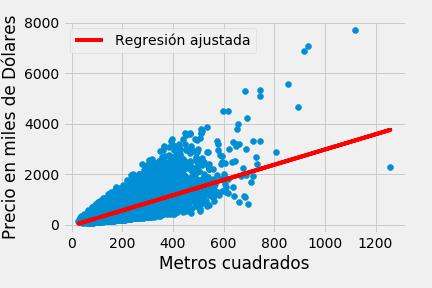
\includegraphics[scale=0.6]{imagenes/linear_fit}
%            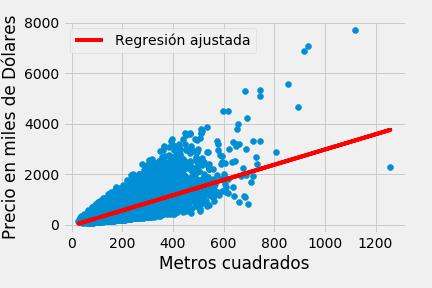
\includegraphics[scale=0.55]{imagenes/linear_fit}
            \caption[Ajuste de regresión lineal]{Ajuste de una regresión lineal a un conjunto de datos de precios de casas\\ Fuente: Elaboración propia}
        \end{figure}
    	
    	\vspace{-10mm}
    	\subsubsection{REGRESIÓN GENERALIZADA}
    		Si se aplica una función $\mathbb{R}^n\mapsto\mathbb{R}$ antes de obtener la predicción, y se optimiza en base a esta definción, se obtienen variantes de la regresión denominados modelos lineales generalizados.
    		
    		Un ejemplo de caso categórico es la regresión logística, pero existen distintos otros modelos como la regresión Poisson o incluso la predicción de una regresión con variable de salida en un rango $(-1, 1)$ definida por una tangente hiperbólica.
    		
    	\subsubsection{MEDIAS MÓVILES EXPONENCIALES}
    		Es un filtro aplicado a una señal o serie de tiempo, con el fin de promediar los valores en un tiempo $t$ de manera ponderada exponencialmente por los términos anteriores de la serie.
    		
    		Se aplica comúnmente para encontrar tendencias de los datos y para suavizar oscilaciones dadas por valores atípicos de poca duración en la señal.
    		
    		Al depender de valores previos de la serie, se calcula de manera recursiva con la fórmula
    		
    		\begin{equation}
    			S_t = \begin{cases}
    				y_0, & t=0\\
    				\alpha y_t + (1 - \alpha)S_{t-1}, & t \ge 1
    			\end{cases}
    		\end{equation}
    	
    		definida por un parámetro $\alpha$ que a mayor valor descarta observaciones antiguas más rápido \citep{10.5555/3002669}.
    	
        % \vspace{-8mm}
        % \begin{center}
        %     Fuente: Elaboración propia
        % \end{center}
    \subsection{CLASIFICACIÓN}
        Cuando la variable respuesta es de tipo categórica, se considera una tarea de clasificación, en que dado un vector de entrada $\mathrm{x_i}$ se debe predecir cuál es la categoría a la que pertenece. \citep{hastie01statisticallearning}
        \subsubsection{REGRESIÓN SOFTMAX}
        Es un modelo lineal generalizado, el cual extiende la idea de la regresión lineal mediante la función de enlace logit multinomial, también llamada softmax, la cual es una generalización de la función sigmoide a múltiples clases, cuyo valor de salida es un vector de probabilidades excluyentes para cada fila de la matriz $\hat{Y}$
        
        \begin{equation}
            Softmax(Z) = \frac{e^{Z}}{\sum_{j=1}^{C} e^{Z_j}}
        \end{equation}
        
        \noindent dónde $Z = \mathbf{X}\cdot\theta$, con $\theta$ ahora de dimensiones $(n \times c)$ siendo $c$ el número de clases, de este modo, mientras mayor el valor de $Z_{i,j}$, mayor es la probabilidad al predecir la clase $j$. \citep{Goodfellow-et-al-2016}
        
        Gráficamente, se interpreta este modelo como el mejor hiperplano que separa el espacio en $c$ partes, donde cada parte contiene las observaciones de su correspondiente clase.
        
        \begin{figure}[H]
            \centering
            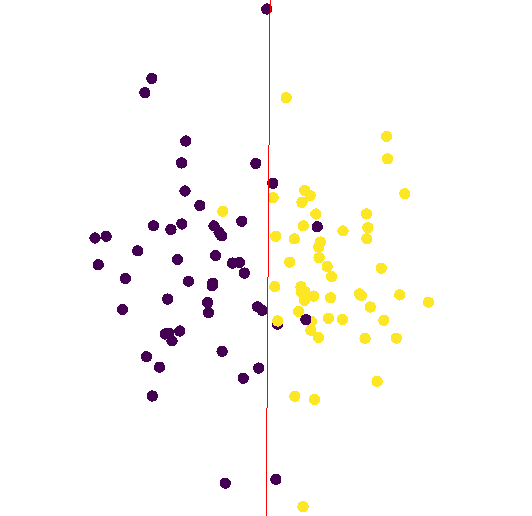
\includegraphics[scale=0.42]{imagenes/logistic_reg}
            \caption[Ajuste de regresión logística]{Ajuste de una regresión logística a un conjunto de datos con 2 clases\\ Fuente: Elaboración propia}
        \end{figure}
        % \vspace{-8mm}
        % \begin{center}
        %     Fuente: Elaboración propia
        % \end{center}
        Debido a la nolinealidad de la función de enlace, los parámetros ya no se pueden estimar de manera analítica, por lo que se debe usar un método iterativo para resolver el sistema, sin embargo, lo más importante y requisito de todos los métodos, es encontrar la derivada de la función de costo con respecto a los parámetros.
        
        Con el fin de tener una mejor medida del error para las probabilidades de las categorías, se usa la función log softmax
        
        \begin{equation}
            \mathcal{L} = -log(\hat{y})
        \end{equation}
        
        \noindent derivando por regla de la cadena $\frac{\partial\mathcal{L}}{\partial \theta} = \frac{\partial\mathcal{L}}{\partial Z} \cdot \frac{\partial Z}{\partial \theta}$, se obtiene
        
        \begin{equation}
            \frac{\partial\mathcal{L}}{\partial \theta} = X' \cdot (\mathbf{\hat{y}} - \mathbf{y})
        \end{equation}
        
        \noindent la derivada requisito para cualquier algoritmo de optimización.
        
    \subsection{DESCENSO DEL GRADIENTE ESTOCÁSTICO}
        Uno de los métodos más utilizados para resolver el sistema y encontrar los parámetros de modelos no lineales. Consiste en particionar el conjunto de datos en pequeños lotes, de modo que en cada iteración, se evalúa la derivada en cada lote y se mueven los valores de los parámetros en dirección al mínimo de la función \citep{hastie01statisticallearning}.
        
        \begin{figure}[H]
            \centering
            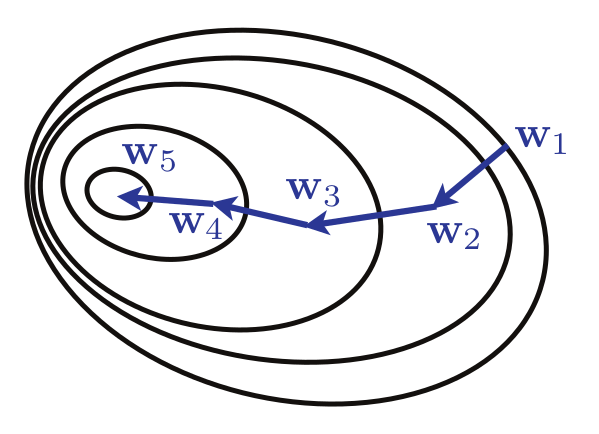
\includegraphics[scale=0.38]{imagenes/sgd}
            \caption[Pasos de los parámetros $W$ en cada iteración camino al mínimo error]{Pasos de los parámetros $W$ en cada iteración camino al mínimo error\\ Fuente: \citep{10.5555/3360093}}
        \end{figure}
      
        {\setstretch{1.0}
        \begin{algorithm}[H]
        	\caption{\textit{Descenso del Gradiente estocástico}}
        	\SetAlgoLined
        	\KwData{$\mathbf{X}:$ Matriz de observaciones}
        	\KwData{$\mathbf{Y}:$ Vector de valores a predecir}
        	\KwData{$\alpha:$ Tamaño del paso de aprendizaje}
        	\KwData{$b:$ Tamaño del lote}
        	\KwData{$f(\mathbf{X}, \theta):$ Función objetivo a optimizar}
        	Inicializar aleatoriamente $\mathbf{\theta}$\\
        	\While{$\mathbf{\theta}$ no converge}{
        		\For{$i$ $\to$ $\frac{m}{b}$}{
        		    $\mathbf{\theta} \leftarrow \mathbf{\theta} - \alpha\cdot \nabla f(\mathbf{X}_i, \theta)$
        		}
        	}
        	\Return $\theta$
        \end{algorithm}
        }
        
        \noindent dónde $\mathbf{\theta} \leftarrow \mathbf{\theta} - \alpha\cdot \nabla f(\mathbf{X}_i, \theta)$ es el gradiente en cada lote.
	\subsection{ADAM}
		Es una mejora del descenso del gradiente, la más utilizada debido a la mayor velocidad de convergencia.
		
		{\setstretch{1.0}
			\begin{algorithm}[H]
				\caption{\textit{Adam}}
				\SetAlgoLined
				\KwData{$\mathbf{X}:$ Matriz de observaciones}
				\KwData{$\mathbf{Y}:$ Vector de valores a predecir}
				\KwData{$\alpha:$ Tamaño del paso de aprendizaje}
				\KwData{$\beta_1$, $\beta_2$ $\in [0, 1)$ parámetros de las medias móviles}
				\KwData{$b:$ Tamaño del lote}
				\KwData{$f(\mathbf{X}, \theta):$ Función objetivo a optimizar}
				Inicializar aleatoriamente $\mathbf{\theta}$\\
				Inicializar en 0 $m$ \tcp*{vector de la media}
				Inicializar en 0 $v$ \tcp*{vector de la varianza}
				$n \leftarrow 0$\\
				\While{$\mathbf{\theta}$ no converge}{
					$n \leftarrow n + 1$\\
					\For{$i$ $\to$ $\frac{n\_observaciones}{b}$}{
						\vspace{1.5mm}
						$g \leftarrow \nabla f(\mathbf{X}_i, \theta)$ \tcp*{gradiente del i-ésimo lote}
						$m \leftarrow \beta_1\cdot m + (1-\beta_1)\cdot g$ \tcp*{MAE de la media}
						$v \leftarrow \beta_2\cdot v + (1-\beta_2)\cdot g\odot g$ \tcp*{MAE de la varianza}
						$\hat{m} \leftarrow \frac{m}{1-\beta_1^n}$ \tcp*{corrección del sesgo}
						$\hat{v} \leftarrow \frac{v}{1-\beta_2^n}$\\
						$\theta \leftarrow \theta - \alpha\cdot\frac{\hat{m}}{\sqrt{\hat{v}}+\varepsilon}$\\
					}
				}
				\Return $\theta$
			\end{algorithm}
		}
	
		El algoritmo aplica dos medias móviles exponenciales, una con parámetro $\beta_1$ para estabilizar las oscilaciones calculando la media del gradiente, y otra con $\beta_2$ estimar la varianza no central, usando la media de los gradientes al cuadrado debido a la relación.
		
		\begin{equation}
			E[X]^2 = E[X^2]	- Var[x]
		\end{equation}
		
		Dado que los momentos estimados son sensibles a la inicialización, se realiza una corrección de sesgo del estadístico estimado
		
		\begin{equation}
			\hat{\bar{X}} = \frac{\bar{X}}{1-\beta_i^n}
		\end{equation}
		
		con $n$ la n-ésima iteración, de esta forma el denominador tiende a $1$ conforme pasan las etapas de optimización.